
\documentclass{report}

\usepackage{graphicx}
\usepackage{xcolor}
\usepackage{hyperref}
\usepackage{listings}

\graphicspath{{img/}}

\title{Firefox WebExtensions security infrastructure}
\date{}
\author{Francesco Pasquali \\Matr. 1933764}


%% DEFINIZIONI
\newcommand{\MComment}[3]{\textcolor{#3}{ \textbf{#1} \textit{#2}}}
\newcommand{\Nota}[1]{\MComment{Nota:}{#1}{olive}}
\newcommand{\Assert}[1]{\MComment{Assert:}{#1}{red}}
\newcommand{\Todo}[1]{\MComment{TODO:}{#1}{brown}}

\newcommand{\code}[1]{\texttt{#1}}

\newcommand{\vuln}{\textit{"vuln"}}

\definecolor{codegreen}{rgb}{0,0.6,0}
\lstdefinestyle{mystyle}{ 
    commentstyle=\color{codegreen},
    basicstyle=\ttfamily\footnotesize,
    breakatwhitespace=false,         
    breaklines=true,                 
    captionpos=b,                    
    keepspaces=true,                 
    numbers=left,                    
    numbersep=5pt,                  
    showspaces=false,                
    showstringspaces=false,
    showtabs=false,                  
    tabsize=2
}
\lstset{style=mystyle}

%% END DEFINIZIONI

%% ARTICOLO
\begin{document}

\maketitle
\tableofcontents
\newpage

\chapter{Introduzione}
    \Nota{Perché i browser?}\\
    I Web Browser Web sono programmi complessi volti a visualizzare contenuti di vario genere
    provenienti dalle fonti piu disparate, dai file locali alle risorse accessibili nell'
    internet, dalle immagini ai linguaggi di scripting. In un mondo sempre piu connesso, i
    browser sono diventati de facto applicazioni necessarie nella vita di tutti i giorni e
    utilizzate da una vastissima comunità di utenti; la loro diffusione unita alla capacità
    di eseguire codice javascript direttamente sulla macchina dell'utente rende i browser
    dei bersagli di interesse per il red-team, aprendo alla possibilità di compromettere un
    grande numero di dispositivi.\\

    \Nota{Perché Firefox?}\\
    Firefox è un Web Browser che in passato ha avuto un'ampia comunità di utenti, noto per
    le politiche a tutela privacy e la storica concorrenza con Internet Explorer


    \Nota{Perché le estensioni?}\\
    Perché è codice scritto da terze parti a cui il browser da accesso ai contenuti web e
    ad API privilegiato normalmente non accessibili dal DOM, queste caratteristiche mi hanno
    indotto ad astrarre le estensioni come una sorta di ponte tra la pagina e il sistema,
    certo le estensioni non sono le uniche componenti del browser a svolgere questo ruolo
    (basti pensare all'interprete html), ma a differenza delle altre esse sono programmabili
    ( e programmate ) da sviluppatori esterni al progetto Firefox e potenzialmente
    ignari sulle misure di sicurezza nello sviluppo web in ambiente browser. 
    Con questi presupposti ho ipotizzato uno scenario in cui l'attaccante abbia la
    possibilità di sfruttare una estensione vulnerabile ad attacchi di tipo html injection
    e sono andato a studiare se e in che modo il browser sia in grado di difendersi
    da tale scenario.


\newpage
\chapter{Metodo}
    \section{Threat model}
        \begin{itemize}
            \item \textbf{Attaccante} Un membro del red-team interessato a compromettere
                il web browser (Firefox) della vittima come parte di una catena di attacco.
                Il suo obbiettivo è ottenere esecuzione di codice Javascript arbitrario che abbia
                accesso agli API interni di Firefox.
                Esso non ha altro modo di interagire con il sistema attaccato se non tramite
                una applicazione web di cui controlla quantomeno il codice dell'interfaccia utente;
                tale applicazione è visitabile attraverso un dominio pubblico ed espone endpoint
                http e/o https.

            \item \textbf{Vittima} Un utente privo di competenze in ambito cybersecurity.
                Esso è stato persuaso ad utilizzare la propria installazione di Firefox
                per visitare il dominio malevolo controllato dall'attaccante.
        \end{itemize}

    \section{Specifiche applicazione e piattaforma}
        Per la mia ricerca ho svolto i test utilizzando l'ultima versione corrente di
        Mozilla Firefox v122.0 installata su MacOS Monterey v12.5 con processore Apple M1.
        Il codice sorgente studiato è stato scaricato dalla repository github ufficiale di mozilla,
        commit b59eed0; ogni menzione contenuta in questo articolo è relativa allo stato del codice
        risalente al suddetto commit. link: \url{https://github.com/JackieSpring/firefox/tree/b59eed054bcd27fbdf7e796ee5993dfb69d47f55}. 
        L'applicazione è stata compilata seguendo le istruzioni riportate sul sito
        ufficiale di mozilla, link: \url{https://firefox-source-docs.mozilla.org/setup/macos_build.html}.

        L'installazione di Firefox utilizzata dalla vittima è l'ultima versione corrente
        del browser ( attualmente Firefox 122.0 ). La vittima ha installato una estensione,
        vulnerabile ad attacchi di code injection, che chiameremo "\textit{vuln}".


    \section{L'estensione \vuln}

        Il manifesto dell'estensione \vuln dichiara tre componenti:
        \begin{itemize}
            \item Un \textbf{Content script} incaricato di ottenere coppie chiave-valore
                e inviarle in background. La coppia viene cercata all'interno della pagina
                e puo anche essere ricevuta attraverso un evento custom "trigger", in
                entrambi i casi la protezione Xray deve essere attenuata esponendo l'estensione.

            \item Un \textbf{Background script} memorizza la coppie ricevuta dal content script 
                in un archivio salvato nel local storage del browser, implementato
                come array di oggetti.

            \item Una \textbf{Sidebar} che visualizza i dati delle coppie nella propria finestra
                inserendoli come testo html.
        \end{itemize}

        I primi due compongono la logica dell'estensione mentre la sidebar funge da front-end ma
        non è l'unica componente visualizzabile, insieme ad essa il manifest permette
        di esporre altre finestre UI che sono i popup e la pagina delle opzioni personalizzata; per
        restringere il campo di studio ho deciso di usare solo una delle tre finestre front-end,
        ho ritenuto la sidebar il giusto candidato per le proprietà del componente:
        \begin{itemize}
            \item Il compartimento Javascript in cui viene eseguito il codice della sidebar
                ha gli stessi permessi di accesso al WebExtensionAPI dello script di background
                soddisfacendo gli obbiettivi di bersaglio del threat model.
            
            \item Il compartimento della finestra viene creato all'apertura della sidebar e rimane
                attivo fino alla chiusura della stessa garantendomi controllo sulla durata
                del suo ciclo di vita; inoltre la sidebar rimane visibile accanto ad ogni tab aperta
                favorendone il debugging;
                
        \end{itemize}

        \subsection{La vulnerabilità}
            La vulnerabilità risiede nella logica della sidebar, nella funzione \code{updateArchiveView}

            \begin{lstlisting}
                keyField.innerHTML = data.key + ": ";
                valField.innerHTML = data.value;
        
                container.appendChild( keyField );
                container.appendChild(valField);
            \end{lstlisting}

            quando gli elementi \code{keyField} e \code{valField} vengono aggiunti all'albero di nodi
            del DOM, il campo \code{.innerHTML} viene valutato come valido codice HTML5 e interpretato,
            se "key" o "value" dovessero contenere tag html essi verranno inseriti nel documento come
            elementi validi (l'unica eccezione è il tag \code{<script>}, questo caso verrà approfondito
            in seguito).

        \section{Workflow dell'estensione}
            \Nota{Questa sezione andrebbe spostata nel capitolo di spiegazione dell'attacco}
            Il content script ottiene dal WebContent un oggetto contenente le proprietà "key" e "value",
            poiché l'oggetto proviene da un compartimento con privilegi minori il content script attenua
            la protezione sull'oggetto per poter leggere le proprietà non native, i dati vengono estratti,
            accorpati ad un messaggio, serializzati e trasmessi sul sistema di messaggi del runtime;
            durante questo passaggio vengono perse proprietà e valori non serializzabili, come le funzioni.
            Alla ricezione di un messaggio lo script in background deserializza l'archivio


\newpage{}
\chapter{L'infrastruttura di sicurezza Firefox}
    Ogni sito internet moderno ha in qualche modo il bisogno di interagire con la rete,
    con uno storage locale, con il file system e con dispositivi audio e video, tutte
    risorse gestite dal sistema operativo, pertanto ogni sito deve poter interagire con
    il sistema operativo della macchina client ma dare questo livello di accesso a codice
    insicuro significa esporre il sistema ad alti rischi di sicurezza per queste ragioni
    il browser deve esporre API che rendano possibili le operazioni richieste dal sito
    senza però compromettere la macchina host.
    Firefox non è direttamente responsabile della sicurezza del sistema, questo aspetto è
    invece gestito da rendering engine Gecko di cui Firefox è il front-end.
    Gecko applica quanto detto separando il codice eseguito in compartimenti
    logici, isolati in processi distinti, realizzando layer di separazione a livello
    applicativo e a livello fisico di sistema operativo.

    \section{Modello processi}
        Il codice che compone Firefox e Gecko non è eseguito sotto un unico processo, diversi servizi
        sono eseguiti in diversi processi per garantire solidità nel caso di fallimenti o 
        compromissioni esterne; si dividono in tre categorie:
        \begin{itemize}
            \item \textbf{Parent Process} è il processo principe nonché padre di tutti gli altri,
                è incaricato di coordinare i processi figlio e gestire la comunicazione tra di essi.
                Visualizza pagine ad alti privilegi come \code{about:preferences} e \code{about:config},
                pertanto ospita un ambiente di esecusione ristretto.

            \item \textbf{Helper Processes} sono processi che ospitano servizi, tra essi vi sono servizi
                di interazione con il file system, con la rete, con le immagini e altri ancora.

            \item \textbf{Content Processes} sono processi usati per renderizzare contenuto web, insieme
                al Parent sono gli unici a poter eseguire codice Javascript. Vengono suddivisi in 
                "remote-type", proprietà che specificano i privilegi di accesso agli API.

        \end{itemize}
        Ci sono molti tipi di Content Process di cui due sono di particolare interesse per la mia ricerca:
        \begin{itemize}
            \item \textbf{WebExtensions Content Process} È utilizzato per caricare pagine
                in background e i subframe delle estensioni web; esiste una sola istanza di
                questo processo ed ha assegnato il remote-type "extension" che garantisce 
                l'accesso al WebExtensionAPI e alla Shared Memory. Tutte le estensioni condvidono
                questo processo e sono visibili tra di loro.

            \item \textbf{Isolated Web Content Process} Sono usati per ospitare contenuti web attribuiti ad un sito,
                il codice web eseguito in questi processi è considerato insicuro e l'accesso diretto agli
                API di sistema non è permesso. Un nuovo web content viene allocato per ogni sito visitato su
                una browser tab, qualsiasi dominio visitato su una tab differente produce un nuovo processo
                Web Content isolato, invece subframe aperti sullo stesso dominio del superframe contenitore
                vengono eseguiti nello stesso processo del super-frame.
        \end{itemize}

    \section{Sicurezza livello script}
        Il codice Javascript eseguito da Gecko non proviene solo da fonti terze come pagine web o estensioni,
        l'interfaccia grafica del browser (Firefox) e la logica sono controllati da moduli javascript ad
        alti privilegi di accesso pertanto gli script web non possono eseguire nello stesso ambiente del
        javascript di sistema. Il modello processi in se potrebbe sembrare una soluzione adeguata, ma se
        script web e di sistema dovessero eseguire nello stesso processo si creerebbe un conflitto, inoltre
        il browser deve poter accedere a oggetti del web content; la separazione in processi è troppo 
        restrittiva per questi utilizzi; inoltre Javascript è un linguaggio a tipizzazione debole, funzionale
        e di cui le strutture di supporto alla programmazione ad oggetti sono modificabili, un esempio dei
        rischi introdotti da questa dinamicità sono gli attacchi di prototype pollution. Il modello di
        separazione dei processi non è sufficiente a gestire proprietà di linguaggio.

        \subsection{Security Policy}
            Una Security Policy è una definizione di che cose significhi "essere sicuro" per un sistema,
            nel caso di Gecko definisce il livello di accesso garantito verso un oggetto da parte di un
            altro oggetto in relazione a due rapporti: di Origine e di Privilegi.
            Gli oggetti dotati di stessa "origine" sono detti \code{"same-origin"} e hanno libero accesso
            alle proprietà, oggetti dotati di "origine" differente sono detti \code{"cross-origin"}
            e hanno accesso molto ristretto alle proprietà dell'altro.\\
            Se l'oggetto acceduto si trova in uno scope di privilegio piu basso allora l'accedente avrà
            permessi di accesso libero ma potrà vedere solo un insieme ristretto di proprietà ma se invece
            l'oggetto acceduto dovesse trovarsi in uno scope con privilegi piu alti allora non otterà 
            alcun privilegio di accesso. Script "privilegiati" possono clonare uno o piu oggetti in
            scope meno "privilegiati".

        \subsection{Same-Origin Policy}
            La Same-Origin Policy è un insieme di regole d'accesso a risorse situate su altre "origini".
            L' "origine" di una risorsa è definita come tripla di protocollo, dominio e porta, due risorse
            che condividono la stessa origine sono dette \code{same-origin}, altrimenti \code{cross-origin}.
            Le restrizioni imposte dalla Same-Origin Policy dipendono dal contesto d'uso:
            \begin{itemize}
                \item \textbf{Rete} Solitamente una risorsa di rete \code{cross-origin} ottiene accesso in
                    scrittura ed embedding mentre la lettura viene proibita, cioé viene reso possibile
                    inviare richieste cross-origin e incorporare risorse esterne ma non è possibile
                    conoscere il contenuto della risposta.
                    Le regole d'accesso di rete \code{cross-origin} possono essere modificate dalla risorsa
                    acceduta tramite header http o tag html \code{meta}.

                \item \textbf{Storage} Gli spazi di archiviazione sono separati e indipendenti per ogni origine

                \item \textbf{Javascript API} Due sono gli oggetti visibili a \code{cross-origin}: \code{window}
                    e \code{location}, di questi solo un sottoinsieme di proprietà è accessibile, tra queste
                    sono notevoli \code{.postMessage} di \code{window} che consente di scambiare dati \code{cross-origin}
                    tra gli script e \code{.href} di \code{location}, accessibile solo in scrittura, permette di
                    redirigere la finestra.
            \end{itemize}

            \subsubsection{Eccezioni}
                Non tutti i protocolli vengono trattati allo stesso modo dalla Same-Origin Policy, le risorse
                caricate da \code{about:blank} o \code{javascript:} sono considerate avere la stessa origine del
                documento che le contiene, mentre l'origine \code{file:///} è trattata come origine opaca cioè
                le risorse ottenute con questo protocollo non sono mai considerate same-origin, nemmeno se
                risiedenti nella stessa directory.

            \subsubsection{Iframe pitfall}
            \Nota{Rimuovere?}
                L'implementazione degli iframe risente di una piccola falla di referenza; quando viene inserito
                nel documento, \code{iframe} incorpora la pagina \code{about:blank} che viene sostituita non
                appena la risorsa è caricata, pertanto lo stesso iframe mostra agli API javascript oggetti con
                origine differente in due momenti diversi.


        \subsection{Compartimenti Javascript}
            I compartimenti sono aree di memoria indipendenti e sono alla base della sicurezza degli script
            in Gecko; ogni oggetto globale e gli oggetti associati alle sue proprietà condividono lo stesso
            compartimento. Gli oggetti memorizzati in un compartimento non sono direttamente accessibili da 
            script appartenente ad un compartimento diverso, la condivisione di oggetti è ottenuta tramite
            oggetti wrapper memorizzati nel compartimento dello script che referenziano l'oggetto originale,
            il grado di accesso fornito dal wrapper verso l'oggetto rappresentato è determinato da Gecko
            secondo la Security Policy.
            I criteri di origine sono valutati considerando come "origine" l'url dell'istanza di \code{window}, 
            che è oggetto globale di ogni compartimento. I criteri di privilegio sono invece determinati
            secondo l'Entità di Sicurezza del compartimento.
            \begin{itemize}
                \item \textbf{Same-Origin} È il caso più comune, all'oggetto accedente viene concesso un
                    wrapper trasparente che garantisce accesso completo all'oggetto richiesto come se 
                    fosse parte dello stesso compartimento. 

                \item \textbf{Cross-Origin} Gecko assegna un wrapper cross-origin che limita l'accesso 
                    secondo la Same-Origin Policy.

                \item \textbf{Privilegio Maggiore} Se lo scope acceduto ha privilegi minori, allora si
                    ottiene un wrapper Xray (di più su Xray Vision in seguito)

                \item \textbf{Privilegio Minore} Se lo scope acceduto ha privilegi maggiori, allora si
                    ottiene un wrapper opaco che nega l'accesso all'oggetto.
            \end{itemize}

        \subsection{Entità di Sicurezza}
            Un Entità di Sicurezza è qualunque entità che puo essere autenticata da un sistema, in Gecko
            esistono quattro entità sulle quali è definita una relazione di sicurezza.
            Per determinare il rapporto tra due entità si verifica se ciascuna sussume l'altra.
            Le quattro entità sono:
            \begin{itemize}
                \item \textbf{Entità di sistema} Supera ogni check di sicurezza, sussume sè stessa e
                    tutte le altre entità. I compartimenti che eseguono codice di sistema sono istanze
                    di questa entità.

                \item \textbf{Entità di Contenuto} È associata ai contenuti web ed è definita 
                    dall'origine del contenuto, sussume ogni altra entità con cui condivida
                    l'origine.

                \item \textbf{Entità Espansa} È definita come una lista di "origini" su cui si ha accesso
                    completo, essa sussume ogni entità che abbia inclusa la propria origine nella lista
                    ma non è sussunta da nessuna di esse.
                    Un esempio di impiego delle entità espanse sono i Content Script delle estensioni che
                    possono accedere al contenuto di più pagine ma non viceversa. In generale l'entità
                    espansa è utilizzata per garantire permessi cross-origin allo script senza però
                    renderlo entità di sistema.

                \item \textbf{Entità Nulla} Fallisce quasi tutti i check e non sussume sè stesso, può
                    essere acceduto solo da un'entità di sistema.
            \end{itemize}
            Le entità non modellizzano solo il livello di privilegio del compartimento ma anche l'origine
            el il test di relazione fornisce le informazioni sufficienti a computare un wrapper secondo
            la Security Policy, infatti se un compartimento sussume l'altro allora deve avere privilegi pari
            o maggiori, se entrambi si sussumano allora sono \code{same-origin}, se nessuno sussume allora
            si tratta di un accesso \code{cross-origin} se invece è uno solo dei due a sussumere allora
            vi è una differenza di privilegi. L'algoritmo di decisione impiegato da Gecko è rappresentato
            in questo grafico:
            \begin{figure}[h]
                \centering                                                  %% centrata
                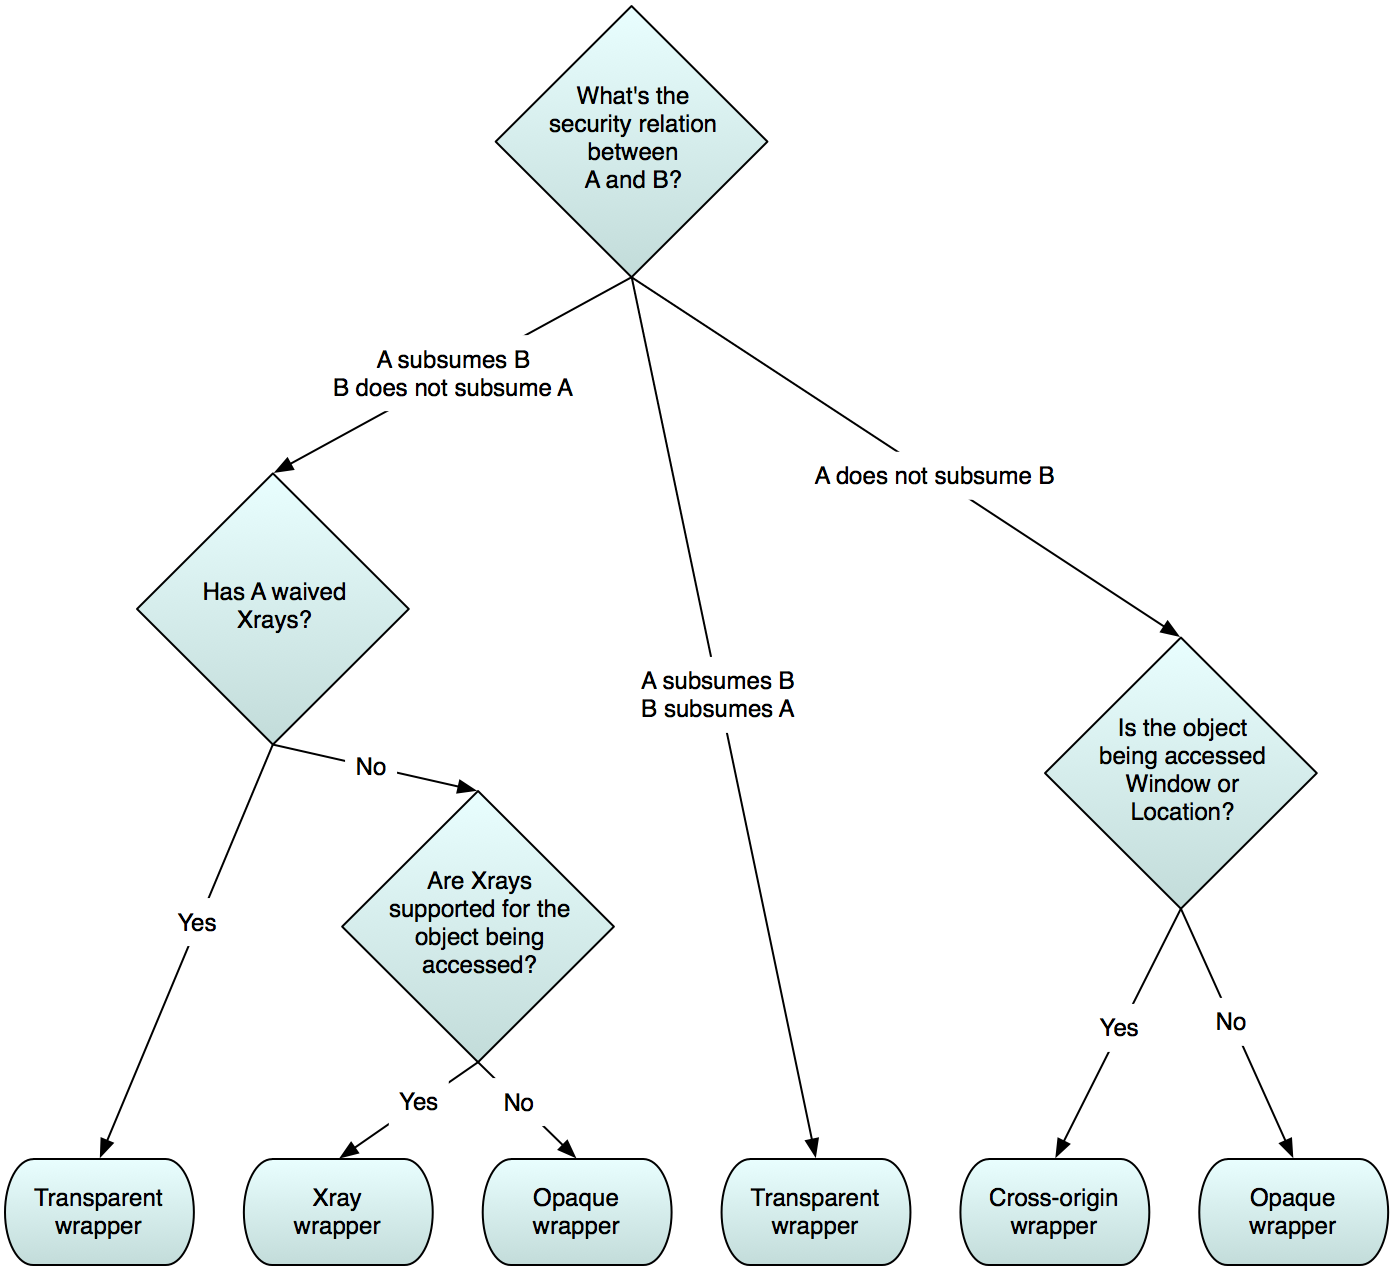
\includegraphics[width=0.5\textwidth]{computing-a-wrapper}  %% il file si chiama "computing-a-wrapper", larga 0.5 volte la largezza del testo
                \caption{Computare un wrapper}                              %% sotto l'immagine c'è una linea descrittiva
                \label{fig:computing-a-wrapper}                             %% potrà essere referenziata da link del documento con questo nome
            \end{figure}

        \subsection{Xray Vision}
            Javascript è un linguaggio molto malleabile il che lo rende imprevedibile in una contesto di
            sicurezza, oggetti provenienti da compartimenti insicuri potrebbero venire adeguatamente
            modificati per ingannare gli script privilegiati ad eseguire codice malevolo; per arginare
            il problema Gecko fa uso dei wrapper Xray, che consentono accesso completo alla forma "base"
            dell'oggetto ignorando le modifiche attuate dagli script, il modo in cui viene ottenuta
            dipende dall'oggetto acceduto.\\
            Gli elementi del DOM sono gli oggetti piu comuni e hanno due implementazioni: 
            una a livello Javascript che "vive" all'interno del proprio compartimento e memorizza lo
            stato corrente dell'oggetto, e una in codice nativo C++ che descrive la forma base
            dell'oggetto, quando il codice privilegiato deve accedere ad un elemento del DOM, gli viene
            restituito un wrapper Xray che mostra le proprietà della rappresentazione nativa. 
            Alcuni oggetti esistono solo nel runtime Javascript, come gli \code{Array} o le \code{Promise},
            allora si restringono le loro proprietà trattandoli come dizionari: metodi, getter e setter 
            sono ignorati per impedire l'esecuzione di codice malevolo mentre il prototype di \code{Object}
            e \code{Array} viene rimpiazzato con il prototipo standard garantendo l'integrità.\\
            Semmai il codice privilegiato avesse bisogno di conoscere lo stato corrente dell'oggetto la
            visione Xray può venire attenuata programmaticamente accedendo alla prorpietà \code{.wrappedJSObject},
            ma a questo punto non si avrebbero piu garanzie di sicurezza su di esso, nè sui "figli".


\chapter{Attaccando l'estensione "vuln"}


\end{document}
%% END ARTICOLO